% compile: $ pdflatex group.tex

\documentclass[a4paper, notoc]{tufte-handout}

\title{Human Computer Interaction\\ Coursework 2 Report}

\author{Group 35}

%\date{1st January 1970} % without \date command, current date is supplied

%\geometry{showframe} % display margins for debugging page layout
\usepackage{appendix}
\usepackage{graphicx} % allow embedded images
\setkeys{Gin}{width=\linewidth,totalheight=\textheight,keepaspectratio}
\graphicspath{{graphics/}} % set of paths to search for images
\usepackage{amsmath}  % extended mathematics
\usepackage{booktabs} % book-quality tables
\usepackage{units}    % non-stacked fractions and better unit spacing
\usepackage{multicol} % multiple column layout facilities
\usepackage{lipsum}   % filler text
\usepackage{fancyvrb} % extended verbatim environments\
\fvset{fontsize=\normalsize}% default font size for fancy-verbatim environments

\let\origdescription\description
\renewenvironment{description}{
  \setlength{\leftmargini}{1.5em}
  \origdescription
  \setlength{\itemindent}{-1.5em}
  \setlength{\labelsep}{\textwidth}
}
{\endlist}


\begin{document}
\maketitle % this prints the handout title, author, and date
\vspace{1em}
\noindent
\begin{tabular}{l r}
  Chris Campbell & s1334028\\
  Karel Kuzmiak  & s1334628\\
  Angus Pearson  & s1311631\\
  Ben Shaw       & s1338564\\
\end{tabular}

%\tableofcontents
%\newpage

%% REQUIREMENTS %%

\section{Design Motivations and Coverage}

% The topic(s) you decided to cover in the website. What kind of information 
% you were trying to convey

\begin{marginfigure}
  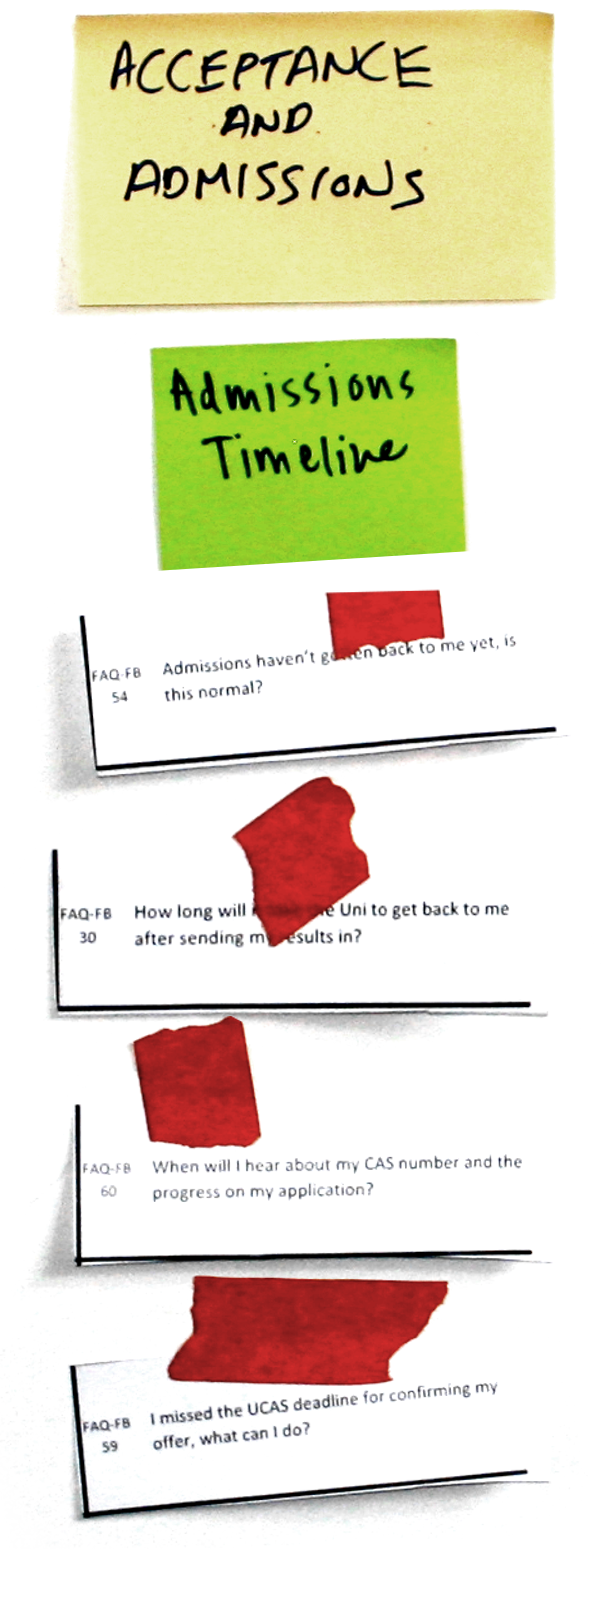
\includegraphics{acceptance_admissions_affinity.png}
  \caption{
    \label{fig:accept-admit-affinity}
    A section of an Affinity Diagram, where all the questions about admissions relate to
    the timing of admissions. Other qustions in the `Acceptance and Admissions' group pertained to
    meeting conditions and the post-decision process.}
\end{marginfigure}

``Produce an interface for students who have \textit{recently} been admitted to the 
University of Edinburgh's School of Informatics''

\vspace{1em}

Looking at the Affinity Diagrams from the HCI Tutorials, it becomes clear there's 
an emergent Linear Chronology to the questions asked. From this it follows that at 
any given time, the questions and information needs a New Student 
may have will be closely related to where they are upon a timeline running towards 
Fresher's week (Illustr. Fig.\ref{fig:accept-admit-affinity}).
 Further to this, a number of tasks required of new students are \textit{``Do once 
and forget''} in nature; it's super important that they do this thing, but once it's done
it doesn't ever need their attention again.

Following from that, we propose a timeline-style interface, where information is arranged 
in cards sequentially along a vertically descending line. Iconography down the timeline 
allows quick scanning and recognition, whith the icon roundalls being clickable, to mark 
the accompanying content card as `done' (Here `done' is rather abstract, meaning completed
or no longer requiring the user's attantion).

As the timeline design is an unfamiliar pattern with most users, a concern is that the 
pointed circles blah afford clicking

% Users aren't affraid to scroll --> Justifies super long single page
% https://www.clicktale.com/academy/blog/unfolding-the-fold-insights-into-webpage-scroll/
%
% 91% of the page-views had a scroll-bar.
% 76% of the page-views with a scroll-bar, were scrolled to some extent.
% 22% of the page-views with a scroll-bar, were scrolled all the way to the bottom.



\section{Usability Analysis}

% Reasoning behind why the website is usable. This section will likely include 
% the outcome of any evaluations you conducted. Unlike the last coursework I do 
% not expect you to do a full formal analysis and description. A few sentences 
% on the method you used is fine. The key is providing reasoning on either why 
% the site is usable, or what you changed to make it so.

\section{Reflection}

% Reflection paragraph: what you have learned from completing this coursework. 
% What worked, what didn't, and if you could go back and do this coursework 
% again what might you do differently the next time.


\section{Tools and Templates}

%% REQUIREMENTS %%
% A list of any tools or templates you used to construct the website.

\begin{description}

\item[Jekyll]
Static site generator (used by GitHub pages) written in Ruby. Supports Markdown for 
content markup and the \textit{SASS} CSS pre-processor.
\\
\href{http://jekyllrb.com/}{http://jekyllrb.com/}

\item[BootStrap]
Web UI framework (CSS, JavaScript) freely available, created by Twitter.
\\
\href{http://getbootstrap.com/}{http://getbootstrap.com/}

\item[FontAwesome]
Web Icon set, freely available.
\\
\href{http://fontawesome.io/}{http://fontawesome.io/}


\item[University of Edinburgh Style Guide]
Fonts -- Serif:- \textit{Crimson Text}, Sans-Serif: \textit{Source Sans Pro} both 
available as \href{https://fonts.google.com/}{Google Web Fonts}.
\\
Colours are taken from 
\href{http://www.ed.ac.uk/communications-marketing/resources}{\textit{Brand Guidelines}} 
and associated pages.
\\



\end{description}




\section*{Mark Allocation}

%% REQUIREMENTS %%

% How the group would like me to allocate marks. Two options: 1) everybody gets 
% the same mark, 2) a clear list of who is responsible for which part of the 
% website or evaluation. In the case of #2 10 points will be marked group wide 
% for the general design of the website and the remaining 40 points will be marked 
% based on the individual portion of the work.



%       ^v^v^v^v^v^v^v^v^v^v^v^v^v^v^v^v^v^v^v^v^v^v^v^v^v^v^v^v^v^v^v^v^v^v^v^


%\bibliography{group}
%\bibliographystyle{plainnat}

\end{document}

